\section{Filesystems and data storage}
\label{sec:fs_data_store}
This section presents how several filesystems used today are structured. \Cref{sec:inodeFSintroduction} presents the idea of \mbox{inode-based} filesystems while \Cref{sec:distributedFSintroducction} gives an introduction to distributed filesystems. Following, in \Cref{sec:data_storage}, the methodology to how data is stored in a storage system and how this information can be used in \gls{FFS} is presented.

\subsection{\mbox{Unix-like} filesystems}
\label{sec:inodeFSintroduction}
A \mbox{Unix-like} filesystem uses a data structure called an \textit{inode}. These inodes are found in an inode table and each inode keeps track of a file's size, blocks used for the file's data, and metadata for the files in the filesystem. A directory simply contains a mapping between filenames and inodes for both the files and directories in a given directory. Given an inode, the filesystem can find information about the file or directory using the inode table. Each inode can contain metadata that might be relevant for the filesystem, such as creation time and last update time. 

\Needspace*{4\baselineskip}
\Cref{fig:inode_diag} shows an example inode filesystem and how it can be visualized. The blocks of an inode entry indicate where in the storage device the data is stored, each block is generally defined as being a certain number of bytes\footnote{typically, 1, 2, 4, or \SI{8}{\kibi\byte}}. \Cref{lst:inode_fs} gives pseudo-code for a simple implementation of an inode, an inode table, and directory entries. 

\begin{figure}[!ht]
	\begin{center}
	  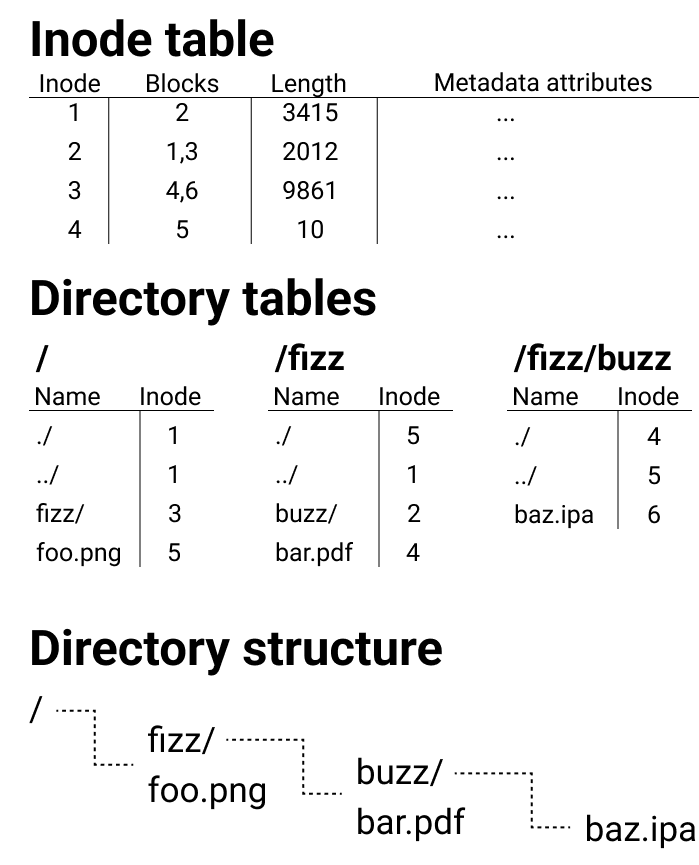
\includegraphics[width=0.5\textwidth]{figures.nosync/inode_diagram.png}
	\end{center}
	\caption{Basic structure of \mbox{inode-based} filesystem}
	\label{fig:inode_diag}
\end{figure}

\begin{minipage}{\linewidth}
\begin{lstlisting}[language=c, caption={Pseudocode of a minimalistic inode filesystem structure}, label=lst:inode_fs]
struct inode_entry {
	int 	length
	int[]	blocks
	// Metadata attributes are defined here
}

struct directory_entry {
	char*   filename
	int     inode
}

// Maps inode_id to an inode_entry
map<int, inode_entry> inode_table

\end{lstlisting}
\end{minipage}

Different filesystems provide different features and limitations. The Extended Filesystem (ext) exists in four different versions: ext, ext2, ext3, and ext4. This filesystem is often used on Linux operating systems. Each iteration brings new features and changes the limitations. For instance, comparing the two latest iterations, ext3 and ext4, ext4 can theoretically store files up to \SI{16}{\tebi\byte} while ext3 can store files up to \SI{2}{\tebi\byte}\,\cite{salterUnderstandingLinuxFilesystems2018}. Additionally, ext4 supports timestamps in units of nanoseconds while ext3 only supports timestamps with a resolution of one second. Additionally, ext4 natively supports encryption at the directory level through the use of the fscrypt \gls{API}\,\cite{FscryptArchWiki}.

\gls{APFS} is a modern filesystem that is used on iPhones and Macs and can store files with a size up to \SI{9}{\exa\byte}\,\cite{igotofferAPFSAppleFile2017}. It supports timestamps in units of nanoseconds and is built to be used on \glspl{SSD}\,\cite{nelsonWhatAPFSDoes}. It also supports modern features that its predecessor Mac OS Extended (HFS+) does not support, such as Snapshots and Space Sharing. \gls{APFS} natively supports encryption of the filesystem volume\,\cite{appleinc.FileSystemFormats}.

\subsection{Distributed filesystems}
\label{sec:distributedFSintroducction}
Filesystems are used to store data, for instance, locally on a hard drive of a computer or in the cloud. Google Drive is an example of a filesystem that enables users to save their data online with up to \SI{15}{\giga\byte} for free\,\cite{CloudStorageWork} using Google's clusters of distributed storage devices. Thnis means that the data is saved on Google's servers which can be located wherever they have data centers\,\cite{DistributedStorageWhat}. Paying customers can have a greater amount of storage using the service. Apple's iCloud and Microsoft's OneDrive are two additional examples of distributed filesystems where users have the option of \mbox{free-tier} and \mbox{paid-tier} storage.

Cloud-based filesystems, as opposed to a filesystem on a physical disk, are accessible from multiple computers and devices without requiring the user to connect a physical disk to the computer. Thus, even if the user loses their computer or if it malfunctions, the data on the \mbox{cloud-based} filesystem can still be accessed, which means that the data could still be recovered. These filesystems are often owned by companies, such as Google Drive and Apple's iCloud, as these big companies can provide reliable storage. This also means that they have their own agenda and policies, and as they are hosting the data, they have the possibility of accessing your data. The data can be encrypted on the filesystem, for instance, by the service provider, but in the case of Google Drive, they have access and control of the encryption and decryption keys which in turn means that they have access and control of the data stored\,\cite{johnsonGoogleDriveSecure2021}. While they mention in their ''Terms of Service'' that the user retains ownership of the data\,\cite{googleGoogleDriveTerms}, they also mention that they can disclose your data for legal reasons and retain the right to review the content uploaded by users\,\cite{googleGoogleTermsService}. Controlling the encryption and decryption keys also enables the possibility of hackers gaining access to your data by attacking Google. Google allows Workspace\footnote{The Google product suit for organizations} organizations to enable client side encryption for Google Drive\,\cite{googleGetStartedEncrypted}, however, it is not available for personal accounts. It is possible to encrypt the data on the client side before uploading files to Google Drive, Google even provides documentation about this\,\cite{googleClientsideEncryptionKeys2023}. iCloud allows users to enable \mbox{end-to-end} encryption for some parts of the service, but not for the whole suite\,\cite{appleinc.ICloudDataSecurity}. For instance, backup data and iCloud drive can be \mbox{end-to-end} encrypted while contacts and iCloud mail cannot.

\subsection{Data storage and encoding}
\label{sec:data_storage}
Different file types have different formats that describe how they should be encoded and decoded; for instance, a JPEG and a PNG file can be used to display visually similar images, but the data they store is different. At the lowest level, storage devices often represent files as a string of binary digits no matter the file type\footnote{There are \mbox{non-binary} storage devices\,\cite{MultistateDataStorage2020}, but this is outside the scope of this thesis.}.

A file can be encoded into text or as an image by representing the bytes in the file as pixel color data and adding a suitable image header for a given image format. This image can, in turn, be posted on, for instance, social media. However, there is a possibility that the social media service compresses the uploaded images, which could lead to data loss and would mean that the decoded data would be different from the encoded data. In this case, the user would be unable to retrieve the original data that was stored unless they were to use methods such as \mbox{error-correcting} codes. These \mbox{error-correcting} codes would have to be stored in an ensured lossless format. For instance, text posts on the \gls{OWS} can be used as long as the posts are not removed or the text is modified.